\chapter{Failure criteria}\label{ch2:title}

Failure criteria aim to describe in the most accurate way rock failure under various states of stress. The most successful criteria are usually a generalization of experimental results, from a combination of axisymmetric and multi-axial tests. Indeed, failure criteria are a theoretical conjecture aimed to describe what is observed from material behavior. In this chapter, a presentation of the mathematical formulation of selected criteria is reviewed.

\section{Introduction}\label{ch2:background}

Many investigators have attempted to develop models or mathematical expression to describe the failure of rock \cite{Labuz2018}. These criteria are usually of an empirical nature and stress based: 

\begin{equation}\label{eq2:rockfail}
    f\left(\sigma_{x x}, \sigma_{y y}, \sigma_{z z}, \sigma_{x y}, \sigma_{y z}, \sigma_{z x}\right)=\text { constant }
\end{equation}

Equation \ref{eq2:rockfail} can be simplified in the case of isotropic materials and the six-parameters stress space can be reduces to three. Indeed, isotropic rock possesses strength properties that are the same in all directions, leading to directional independence. Therefore, the function can then be written in terms of principal stresses: 

\begin{equation}\label{eq2:fsigconst}
    f\left(\sigma_{I}, \sigma_{II}, \sigma_{III} \right)=\text { constant }
\end{equation}

where $\sigma_{I}$, $\sigma_{II}$ and $\sigma_{III}$ are the major, intermediate and minor principal stresses. In addition, other stress invariants can be used:

\begin{equation}\label{eq2:fijjconst}
    f\left(I_{1}, J_{2}, J_{3} \right)=\text { constant }
\end{equation}

$I_{1}$ is the first invariant of the stress tensor $\sigma_{ij}$, $J_{2}$ and $J_{3}$ are respectively, the second and third invariants of the deviatoric stress tensor $S_{ij}=\sigma_{ij}-p\delta_{ij}$: 

\begin{equation}
   I_1 = \sigma_{I} + \sigma_{II} + \sigma_{III}
\end{equation}
\begin{equation}
    J_{2} = \frac{1}{6}\left[\left(\sigma_{I}-\sigma_{I I}\right)^{2}+\left(\sigma_{I I}-\sigma_{I I I}\right)^{2}+\left(\sigma_{I I I}-\sigma_{I}\right)^{2}\right]
\end{equation}
\begin{equation}
    J_{3} = \left(\sigma_{I}-p\right)\left(\sigma_{I I}-p\right)\left(\sigma_{III}-p\right)
\end{equation}

Three others can be defined, and will be used in this thesis: the mean stress $p$ , the deviatoric stress $q$ and the Lode angle $\theta$:

\begin{equation} \label{eq2:fpqtconst}
    f(p,q,\theta) = \text{constant}
\end{equation}
with
\begin{equation} \label{eq2:peq}
    p=\frac{I_{1}}{3}=\frac{\sigma_{I}+\sigma_{II}+\sigma_{III}}{3}
\end{equation}

\begin{equation}\label{eq2:qeq}
    q=\sqrt{3 J_{2}}=\frac{1}{6} \sqrt{\left[\left(\sigma_{I}-\sigma_{II}\right)^{2}+\left(\sigma_{II}-\sigma_{III}\right)^{2}+\left(\sigma_{III}-\sigma_{I}\right)^{2}\right]}
\end{equation}

\begin{equation}\label{eq2:theta}
    \theta=\frac{1}{3} \arccos \left(\frac{3 \sqrt{3}}{2} \frac{J_{3}}{J_{2}^{3 / 2}}\right)=\arctan \left[\frac{\sqrt{3}\left(\sigma_{II}-\sigma_{III}\right)}{2 \sigma_{I}-\sigma_{II}-\sigma_{III}}\right]
\end{equation}

The Lode angle is a measure of the stress state: $0^{\circ} \leq \theta \leq 60^{\circ}$ , particularly $\theta = 0^{\circ}$  for axisymmetric compression $\sigma_{II} = \sigma_{III} $ and $\theta = 60^{\circ}$ in the case of axisymmetric extension ($\sigma_{II} = \sigma_{I} $). 

Equations \ref{eq2:fsigconst}, \ref{eq2:fijjconst} and \ref{eq2:fpqtconst} suggest that the failure surface and consequently the failure criterion has a three-dimensional nature. Indeed, depending on the stress ordering, failure criteria describe six surfaces in a three-dimensional  $\sigma_1 -\sigma_2 -\sigma_3$  space: (i) $\sigma_1 \geq \sigma_2 \geq \sigma_3$, (ii) $\sigma_2 \geq \sigma_1 \geq \sigma_3$, (iii) $\sigma_2 \geq \sigma_3 \geq \sigma_1$, (iv) $\sigma_3 \geq \sigma_2 \geq \sigma_1$,(v) $\sigma_3 \geq \sigma_1 \geq \sigma_2$, (vi) $\sigma_1 \geq \sigma_3 \geq \sigma_1$. For example, a linear criterion, written in terms of the three principal stresses, $\sigma_I$, $\sigma_{II}$, $\sigma_{III}$, shows a pyramidal shape where the planes have a common vertex $V_0$ (the theoretical isotropic tensile strength), which is located on the tension side of the space (see Figure \ref{fig2:pyramid}a).  

\begin{figure}[tb]
    \centering
    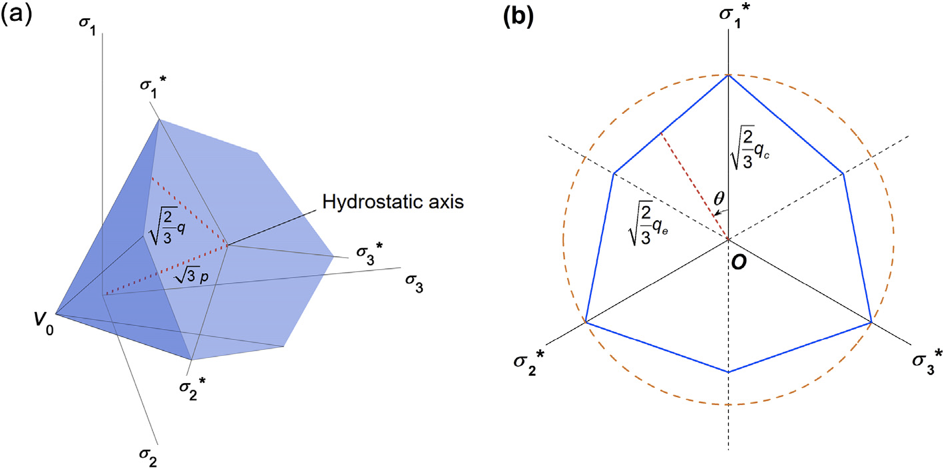
\includegraphics[width=\columnwidth]{ch2/pyramid.png}
    \caption{Failure surface in (a) the principal stress space and (b) the $\pi$-plane \cite[Labuz 2018]{Labuz2018}}
    \label{fig2:pyramid}
\end{figure}

Although the three-dimensional representation of the failure surface is the most complete, other views are often used. For example, two-dimensional coordinates systems such as $(\sigma_3 -\sigma_1)$, $(p-q)$ plane and the $\pi$-plane are simple to view.  

The $\pi$-plane. is a section of the failure surface in the principal stress space, perpendicular to the hydrostatic axis. It is also called the equipressure plane, as the mean stress is constant over the plane. Moreover, the axes $(\sigma_1^*,\sigma_2^*,\sigma_3^*)$ are the projection of the coordinate axis on the $\pi$-plane (cf. \ref{fig2:pyramid}b.). Each point in principal stress space can be represented in polar coordinates in this plane. As the mean stress is constant over the $\pi$-plane, the point is at a distance $r$ from the origin of the hydrostatic axis and oriented at the Lodge angle $\theta$ from the  $\sigma_1^*$ axis. Then the principal coordinates of the same point on the $\pi$-plane can be written as: 

\begin{align}
    \sigma_1 &= p + \frac{\sqrt{6}}{3}r\cos\left(\theta\right) \label{eq2:sig1}\\
    \sigma_2 &= p - \frac{\sqrt{6}}{3}r\sin\left(\frac{\pi}{6}-\theta\right)\\
    \sigma_3 &= p - \frac{\sqrt{6}}{3}r\sin\left(\frac{\pi}{6}+\theta\right) \label{eq2:sig3}
\end{align}

In the next sections, selected failure criteria will be presented along with their formulation in each coordinates system. 

\section{Review}
\subsection{Mohr-Coulomb criterion}

The Mohr-Coulomb failure criterion (MC) is the most popular and widely used criterion. It provides a relationship between the shear stress and normal stress $\sigma$ acting on the failure plane. The failure envelope may be represented using two material parameters known as the internal failure angle $\theta$ and the cohesion $c$ :

\begin{equation}\label{eq2:mc_gene}
    \tau = \sigma \tan \phi + c
\end{equation}

The Mohr-Coulomb failure criterion does not consider the effect of the intermediate principal stress. The shear and normal stresses may be written in terms of the major and minor principal stresses: 

\begin{equation}\label{eq2:tau}
    \tau = \frac{\sigma_I - \sigma_{III}}{2} \cos \phi
\end{equation}

\begin{equation}\label{eq2:sigma}
    \sigma = \frac{\sigma_I + \sigma_{III}}{2} - \frac{\sigma_I - \sigma_{III}}{2} \sin \phi
\end{equation}

Substitution of Equations \ref{eq2:tau} and \ref{eq2:sigma} in Equation \ref{eq2:mc_gene} leads to a form of the Mohr-Coulomb failure criterion in terms of the major and minor principal stresses:

\begin{equation} \label{eq2:MCfinalform}
    \sigma_{I}=\frac{1+\sin \phi}{1-\sin \phi} \sigma_{I I I}+\frac{2 c \cos \phi}{1-\sin \phi}
\end{equation}

or alternatively

\begin{equation}\label{eq2:MCcondenseform}
    \sigma_I = K_p \sigma_{III} + C_0
\end{equation}

where $K_p$ is the slope of the failure surface in $(\sigma_3 -\sigma_1)$ plane and $C_0$ is the uniaxial compression strength of the rock. 

\subsubsection{Mohr-Coulomb in the \texorpdfstring{$(\sigma_3 -\sigma_1)$}{sigma 3 - sigma 1} plane}

Fig \ref{fig2:mc_sig1sig3} presents the graphical construction of Mohr-Coulomb envelope in the $(\sigma_3 -\sigma_1)$ plane. The common vertex of the failure surfaces in extension and compression can be expressed using $\sigma_I = \sigma_{III} = -V_0$ :

\begin{equation}\label{eq2:MC_Vo}
    V_0 = \frac{C_0}{K_p-1}
\end{equation}


\begin{figure}[tb]
    \centering
    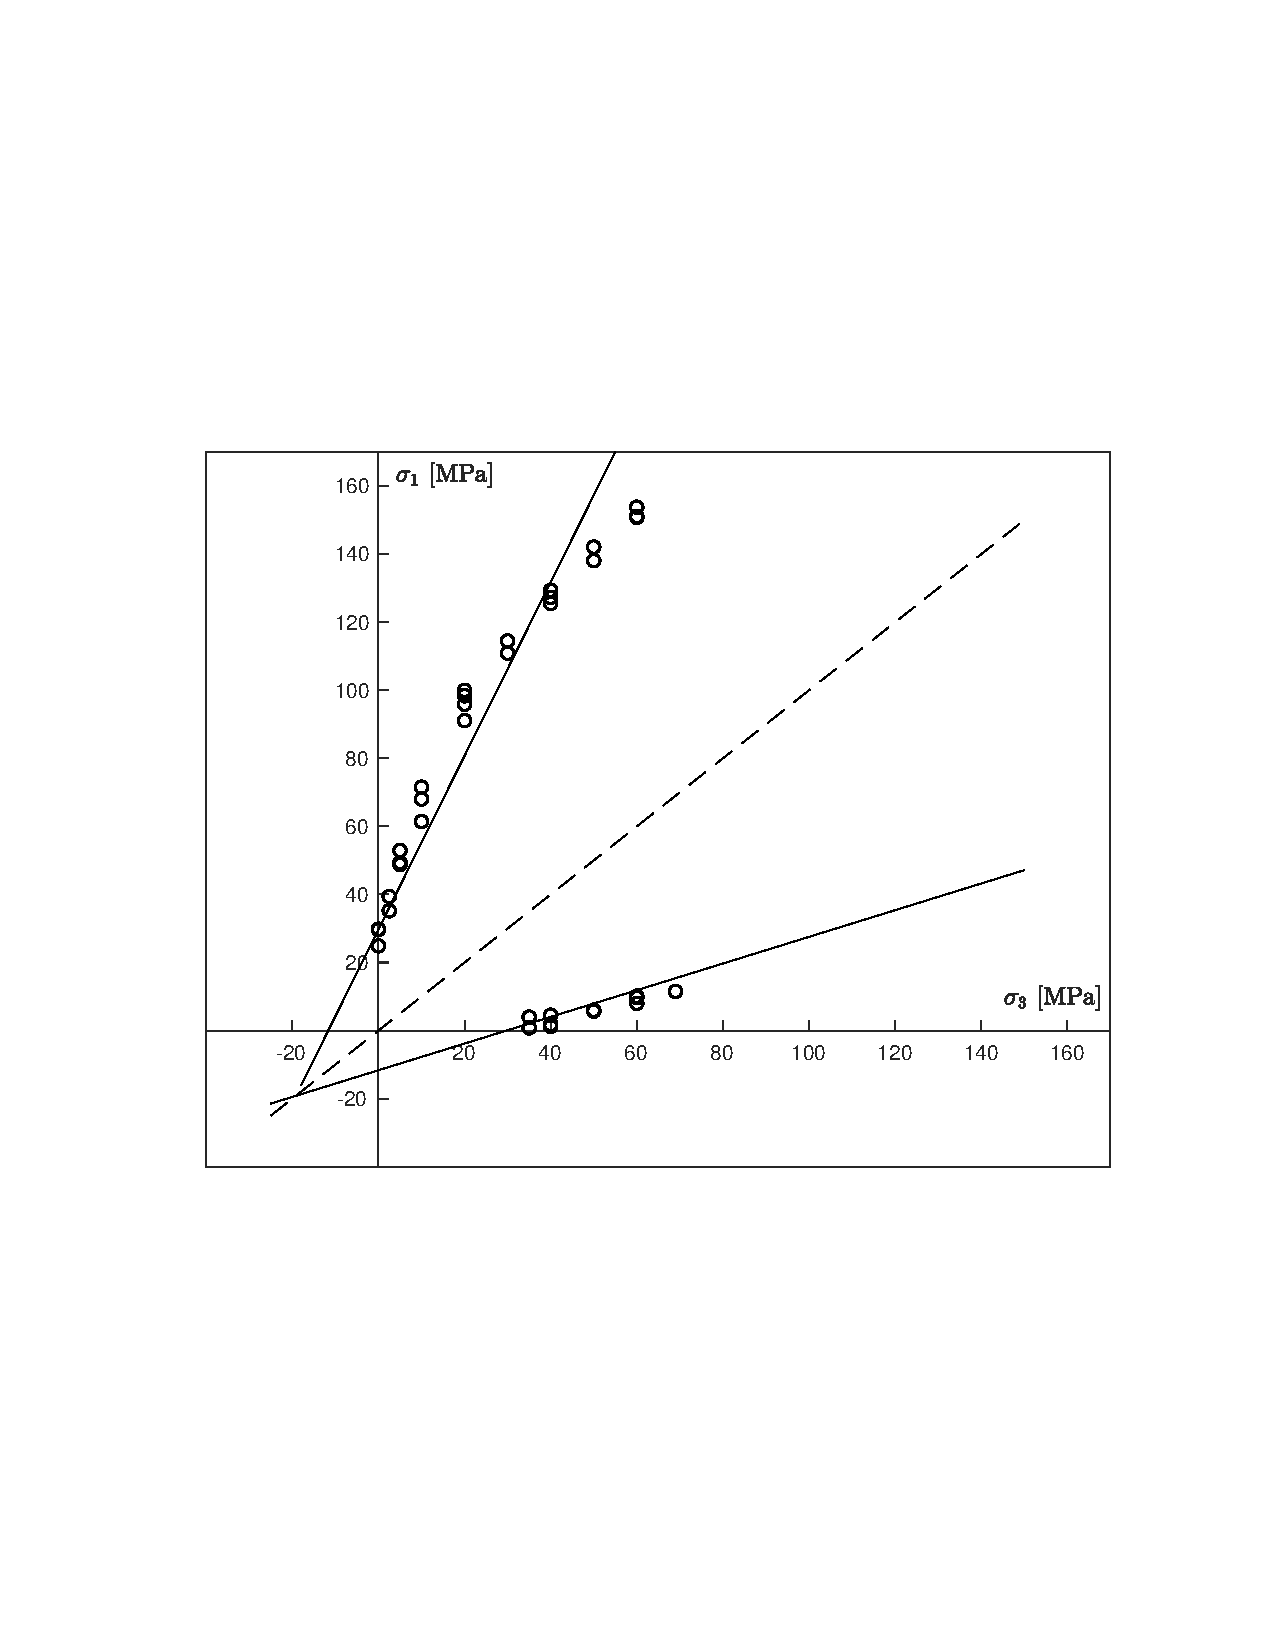
\includegraphics[width=\columnwidth]{ch2/mc_sig1sig3}
    \caption{Mohr-Coulomb criterion failure surface in  $(\sigma_3 -\sigma_1)$ plane}
    \label{fig2:mc_sig1sig3}
\end{figure}

As Mohr-Coulomb does not consider the intermediate stress effect, it may be conveniently used to represent the failure for rocks subjected to stress states that may be replicated in axisymmetric triaxial tests.

Conventional (axisymmetric) Triaxial Compression (CTC): 

\begin{align}
    \sigma_I &= \sigma_a \\
    \sigma_{III} &= \sigma_r\\
    \sigma_{II} = \sigma_{III} &= \sigma_r
\end{align}

Conventional (axisymmetric) Triaxial Extension (CTE):

\begin{align}
    \sigma_I &= \sigma_r \\
    \sigma_{III} &= \sigma_a\\
    \sigma_{II} = \sigma_{I} &= \sigma_r
\end{align}

\subsubsection{Mohr-Coulomb in the \texorpdfstring{$(p - q)$}{p - q} plane} \label{ch2:MC-pq}

The Mohr-Coulomb model can also be represented in $(p-q)$ plane. For example, in axisymmetric triaxial compression, Equations \ref{eq2:peq} and \ref{eq2:qeq} can be written as: 

\begin{align}
    p &= \frac{\sigma_a+2\sigma_r}{2} \label{eq2:p2} \\
    q &= \sigma_a - \sigma_r \label{eq2:q2}
\end{align}

By rearranging Equation \ref{eq2:MCfinalform} and incorporating the conditions for CTC, Mohr-Coulomb criterion becomes:

\begin{equation}\label{eq2:MCcrit}
    \left(\sigma_a - \sigma_r\right) = \left(\sigma_a+\sigma_r\right)\sin \phi + 2 c\cos \phi
\end{equation}

Expanding and substituting Equation \ref{eq2:p2} and \ref{eq2:p2} into \ref{eq2:MCcrit}, the following equation is obtained:: 

\begin{equation}
    q_c(3-\sin \phi) = 6p \sin \phi + 6 c\cos \phi
\end{equation}

Finally, the Mohr-Coulomb failure surface formulation in the $(p-q)$ plane is defined by Equation \ref{eq2:q-CTC} for CTC:

\begin{equation}\label{eq2:q-CTC}
    q_c=\frac{6 \sin \phi}{3-\sin \phi} p+\frac{6 \operatorname{ccos} \phi}{3-\sin \phi} 
\end{equation}

Following the same approach as that for CTC, the M-C criterion for CTE may be written as:
\begin{equation}\label{eq2:q-CTE}
    q_e=\frac{6 \sin \phi}{3+\sin \phi} p+\frac{6 c \cos \phi}{3+\sin \phi}
\end{equation}

or in the condensed form: 

\begin{equation}\label{MC_q}
    q = m_{c,e} p + b_{c,e}
\end{equation}

where $c$ and $e$  defines $m$ and $b$ for compression or extension surfaces:

\begin{equation}\label{eq2:MC_mc_q}
    m_c=\frac{6 \sin \phi}{3-\sin \phi} 
\end{equation}
\begin{equation}\label{eq2:MC_me_q}
    m_e=\frac{6 \sin \phi}{3+\sin \phi} 
\end{equation}
\begin{equation}\label{eq2:MC_bc_q}
    b_c=\frac{6 c \cos \phi}{3-\sin \phi}
\end{equation}
\begin{equation}\label{eq2:MC_be_q}
    b_e=\frac{6 c \cos \phi}{3+\sin \phi}
\end{equation}

Figure \ref{fig2:mc_pq} presents the graphical construction of the failure surfaces in the  $(p-q)$plane. In order to distinguish compression from extension data, the failure surface in extension is shown using a negative deviatoric stress $-q$. 

\begin{figure}[tb]
    \centering
    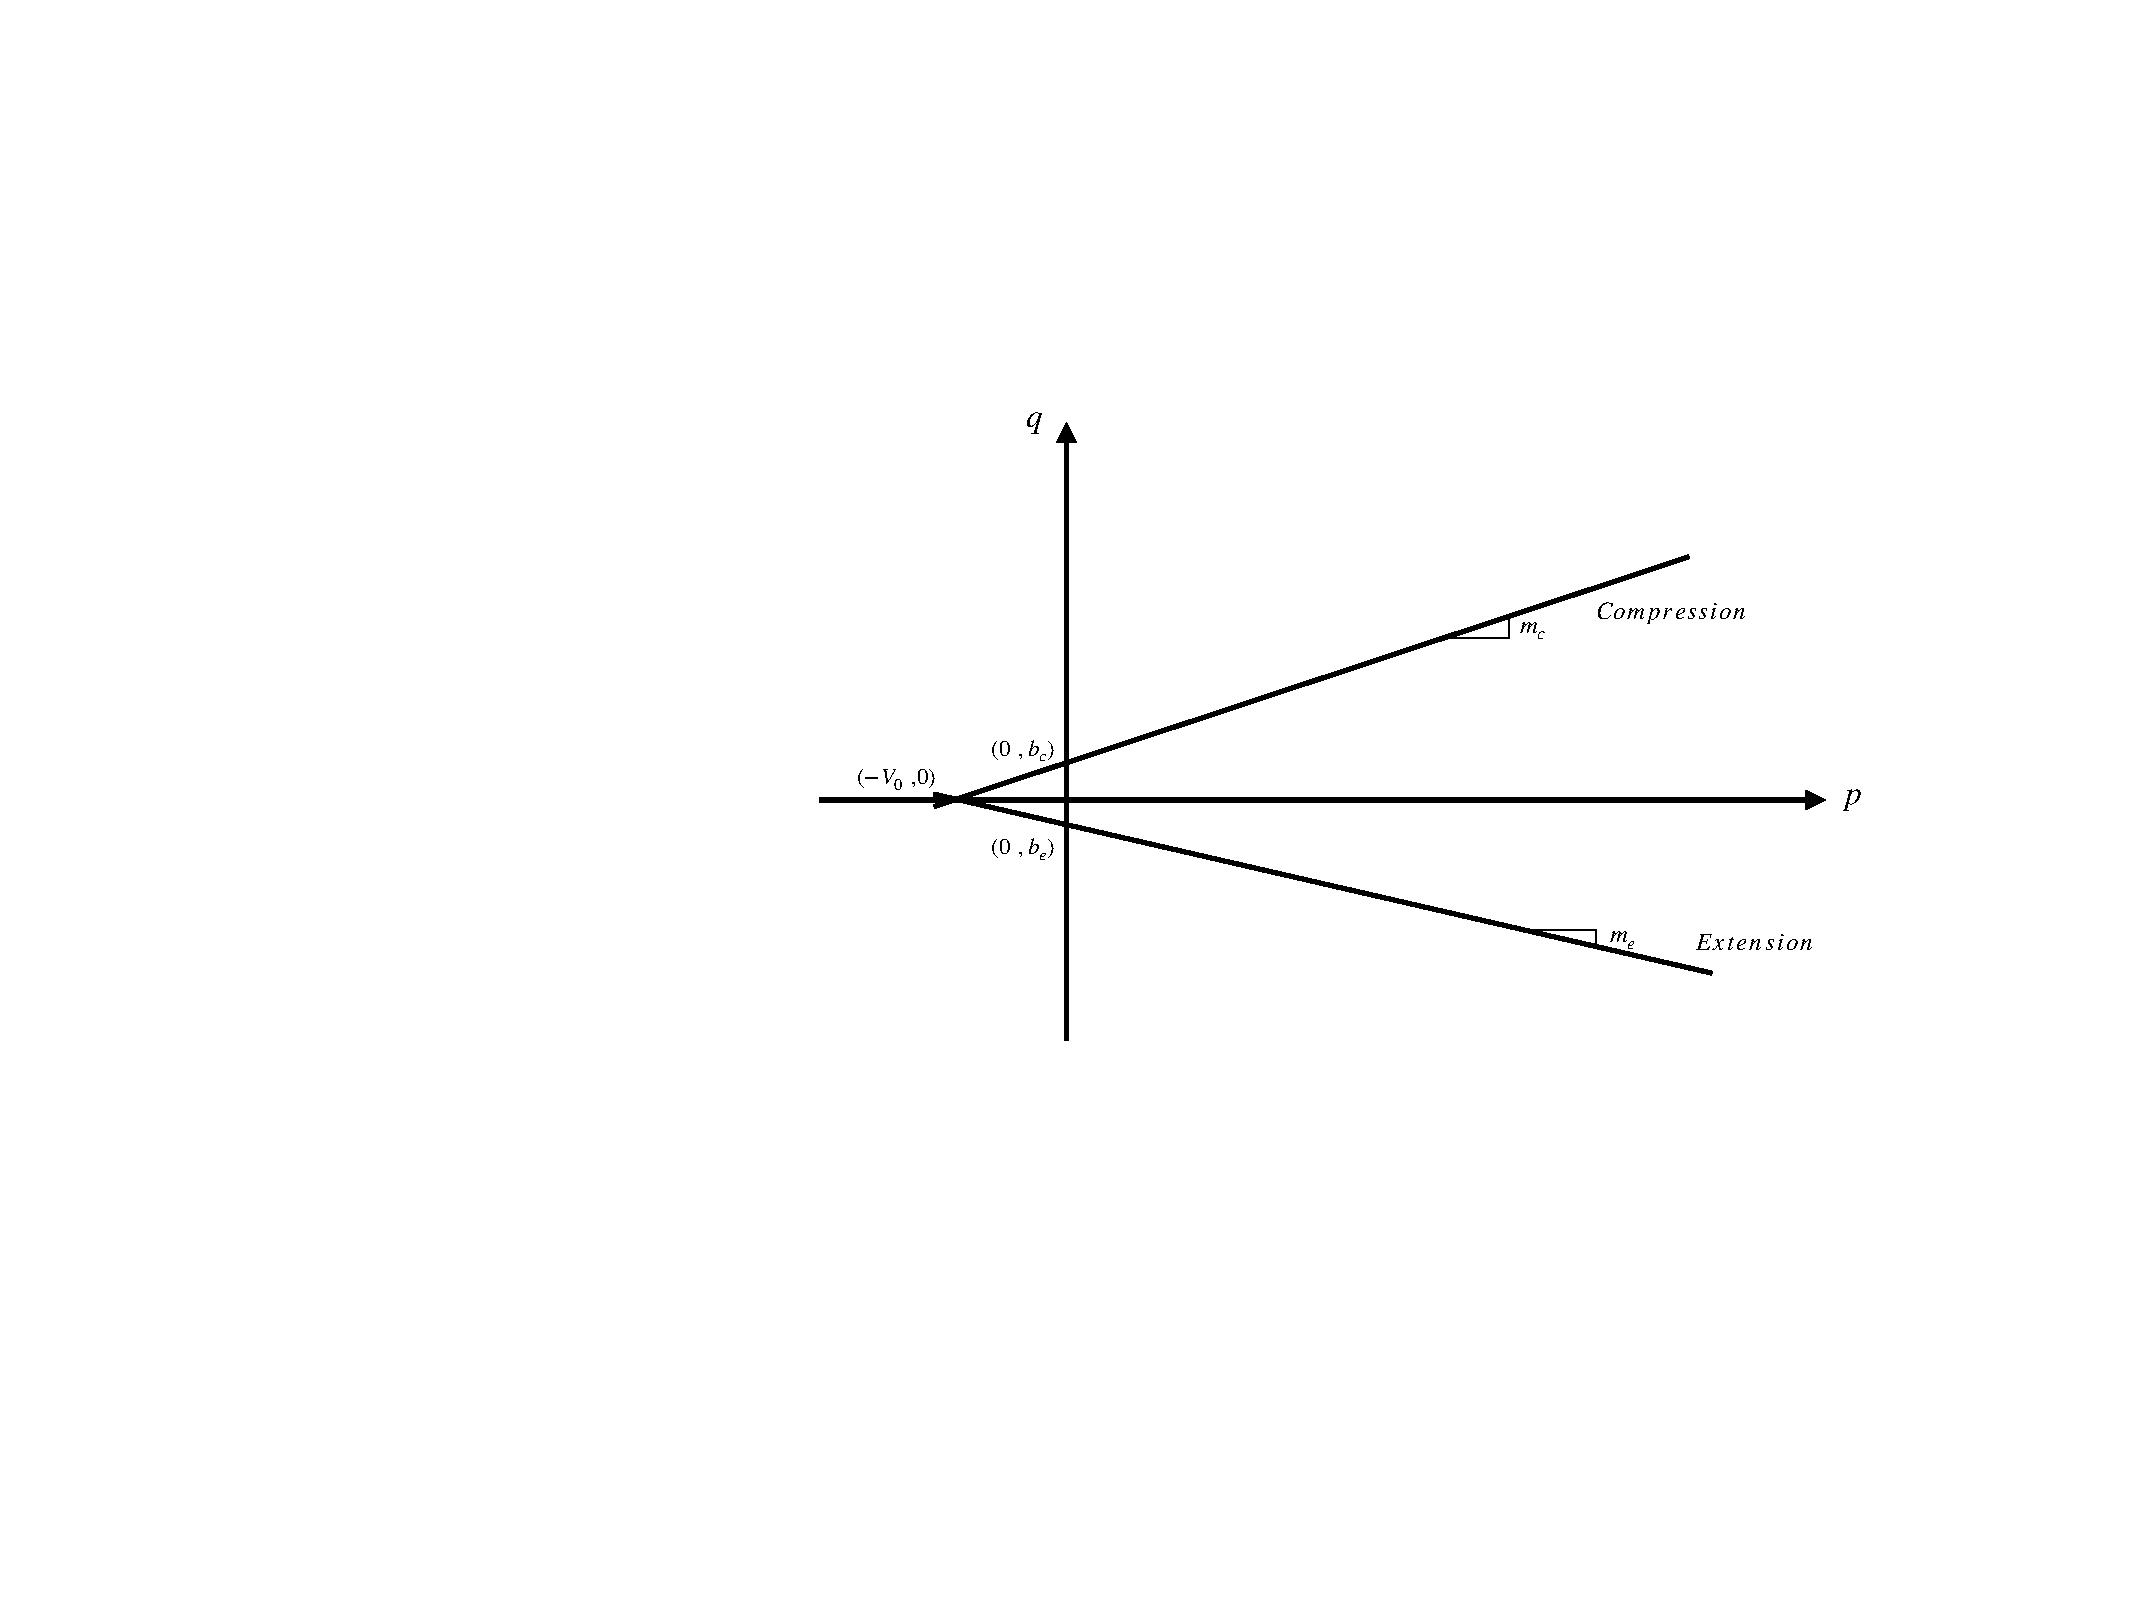
\includegraphics[width=\columnwidth]{ch2/mc_pq}
    \caption{Schematic representation of Mohr-Coulomb criterion failure surface in  $(p-s)$plane}
    \label{fig2:mc_pq}
\end{figure} 

\subsubsection{Mohr-Coulomb in the \texorpdfstring{$\pi$}{pi}-plane}\label{ch2:MC_pi}

The Mohr-Coulomb failure envelope in the $\pi$-plane is presented in Figure \ref{fig2:mc_pi}. The failure surfaces can be obtained by inserting Equation \ref{eq2:sig1} and \ref{eq2:sig3} in the criterion formulation defined by \ref{eq2:MCcondenseform}. The obtained expressions and their development are presented in APPENDIX B REF{APPENDIX B}. 

\begin{figure}[tb]
    \centering
    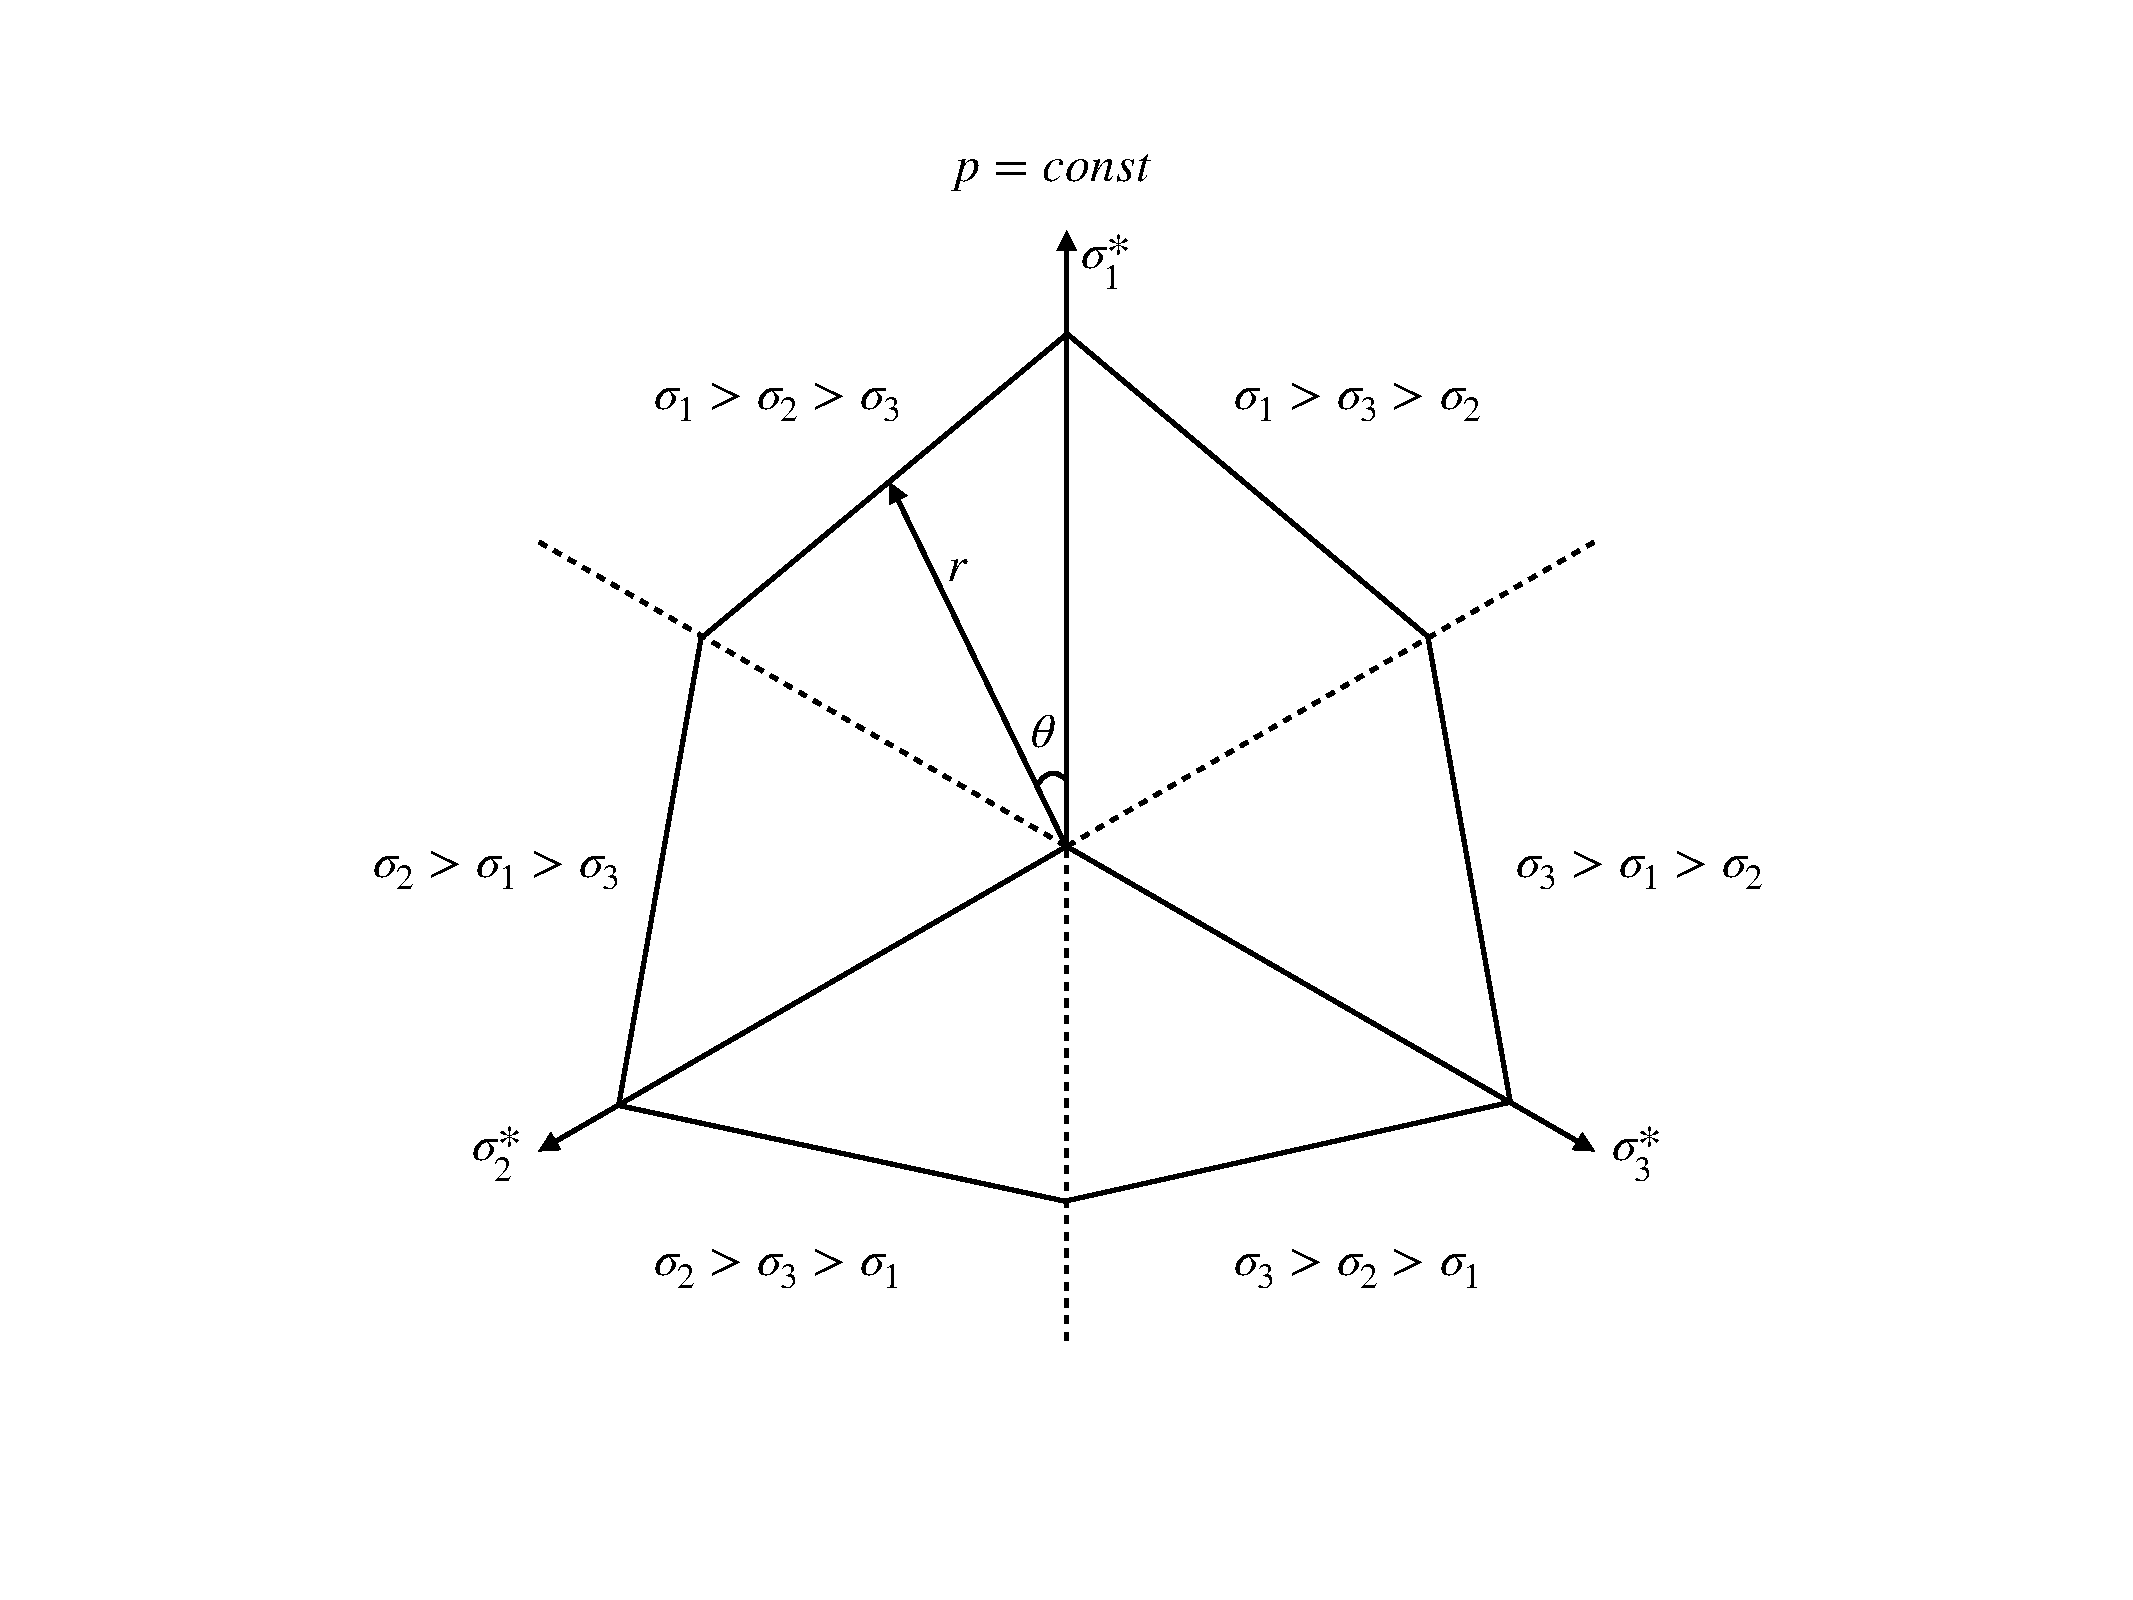
\includegraphics[width=\columnwidth]{ch2/mc_pi}
    \caption{Schematic representation of Mohr-Coulomb criterion failure surface in  $\pi$plane}
    \label{fig2:mc_pi}
\end{figure} 

\subsection{Hoek-Brown criterion}

The Hoek-Brown (HB) criterion is a non-linear model for isotropic rocks that does not account for the intermediate principal stress. The criterion may be written as:

\begin{equation}\label{eq2:HB-crit}
    \sigma_{I}=\sigma_{III}+C_{0} \sqrt{m \frac{\sigma_{III}}{C_{0}}+s}
\end{equation}

Hoek and Brown (1980) \cite{Hoek1980} define $m$ and $s$  as constants that depends on the rock type and “blockiness”. The constant s characterizes the initial state of the tested rock. For intact rock, $s=1.0$ and the strength parameter $m$ is an empirical fitting parameter chosen depending on the rock type.  

\subsubsection{Hoek-Brown in the \texorpdfstring{$(\sigma_3 -\sigma_1)$}{sigma 3 - sigma 1} plane}

In $(\sigma_3 -\sigma_1)$ coordinate system, and for the axisymmetric triaxial compression tests, the Hoek-Brown criterion may be written as:

\begin{equation}\label{eq2:HBsig1_CTC}
    \sigma_{a}=\sigma_{r}+C_{0} \sqrt{m \frac{\sigma_{r}}{C_{0}}+1}
\end{equation}

Similarly, the formulation for axisymmetric triaxial extension is written as:

\begin{equation}\label{eq2:HBsig1_CTE}
    \sigma_{a}=\sigma_{r} - \frac{\sqrt{4 m C_{0} \sigma_{r}+m^{2} C_{0}^{2}+4 C_{0}^{2}}-m C_{0}}{2}
\end{equation}

From Equation \ref{eq2:HBsig1_CTC}, the theoretical isotropic tensile strength $V_0$ can be expressed as a function of the uniaxial compression strength $C_0$, using : $\sigma_a = \sigma_r = -V_0$:

\begin{equation}
    V_0 = \frac{C_0}{m}
\end{equation}

Figure \ref{fig2:hb_sig1sig3} presents the Hoek-Brown failure surfaces in the $(\sigma_3 -\sigma_1)$ coordinates system. 

\begin{figure}[tb]
    \centering
    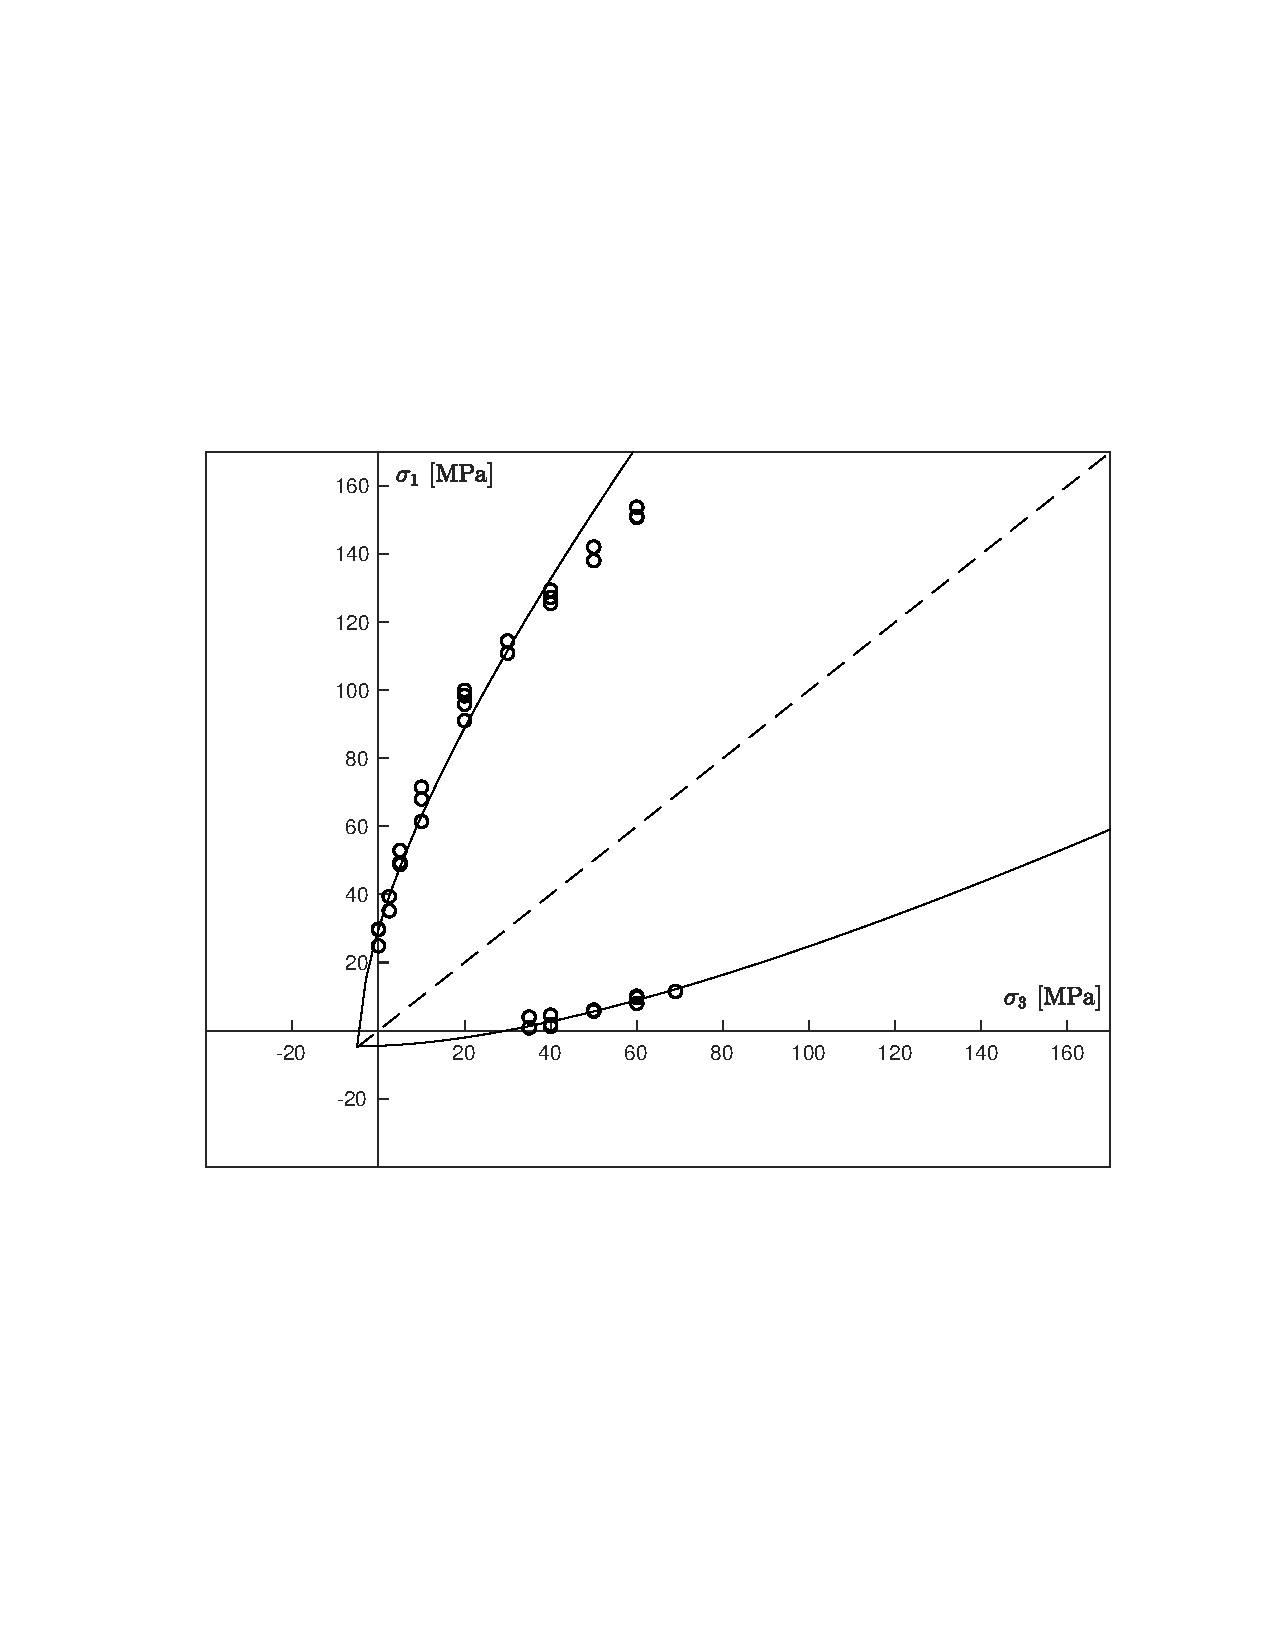
\includegraphics[width=0.8\columnwidth]{ch2/hb_sig1sig3}
    \caption{Schematic representation of Hoek-Brown criterion failure surface in $(\sigma_3 -\sigma_1)$ plane.}
    \label{fig2:hb_sig1sig3}
\end{figure} 

\subsubsection{Hoek-Brown in the \texorpdfstring{$(p-q)$}{p-q} plane}

Hoek-Brown criterion may also be expressed with the stress invariants $p$ and $q$. By rearranging Equation \ref{eq2:HB-crit} the formulation becomes:

\begin{equation}\label{eq2:HB-crit-pq}
    \left(\sigma_{I}-\sigma_{III}\right)^{2}=C_{0}^{2}\left(m \frac{\sigma_{III}}{C_{0}}+s\right)
\end{equation}

By rearranging and inserting $p$  and $q$ in Equation \ref{eq2:HB-crit-pq}, implicit formulation for CTC and CTE are obtained. Equation \ref{eq2:HB-q-CTC} for compression and \ref{eq2:HB-q-CTE} for extension describe Hoek-Brown criterion after solving roots of the implicit expressions:  


\begin{align}
    q_c&=\frac{1}{6}\left(\pm \sqrt{C_{0}} \sqrt{C_{0} m^{2}+36 C_{0}+36 m p}-C_{0} m\right) \label{eq2:HB-q-CTC} \\
    q_e&=\frac{1}{3}\left(\pm \sqrt{C_{0}^{2} m^{2}+9 C_{0}^{2}+9 C_{0} m p}+C_{0} m\right) \label{eq2:HB-q-CTE}
\end{align}

The Hoek-Brown criterion surface fitting in the $(p-q)$ plane is presented in Figure \ref{fig2:hb_pq}, where the positive root of Equation \ref{eq2:HB-q-CTC} and the negative root of Equation \ref{eq2:HB-q-CTE} are considered.

\begin{figure}[tb]
    \centering
    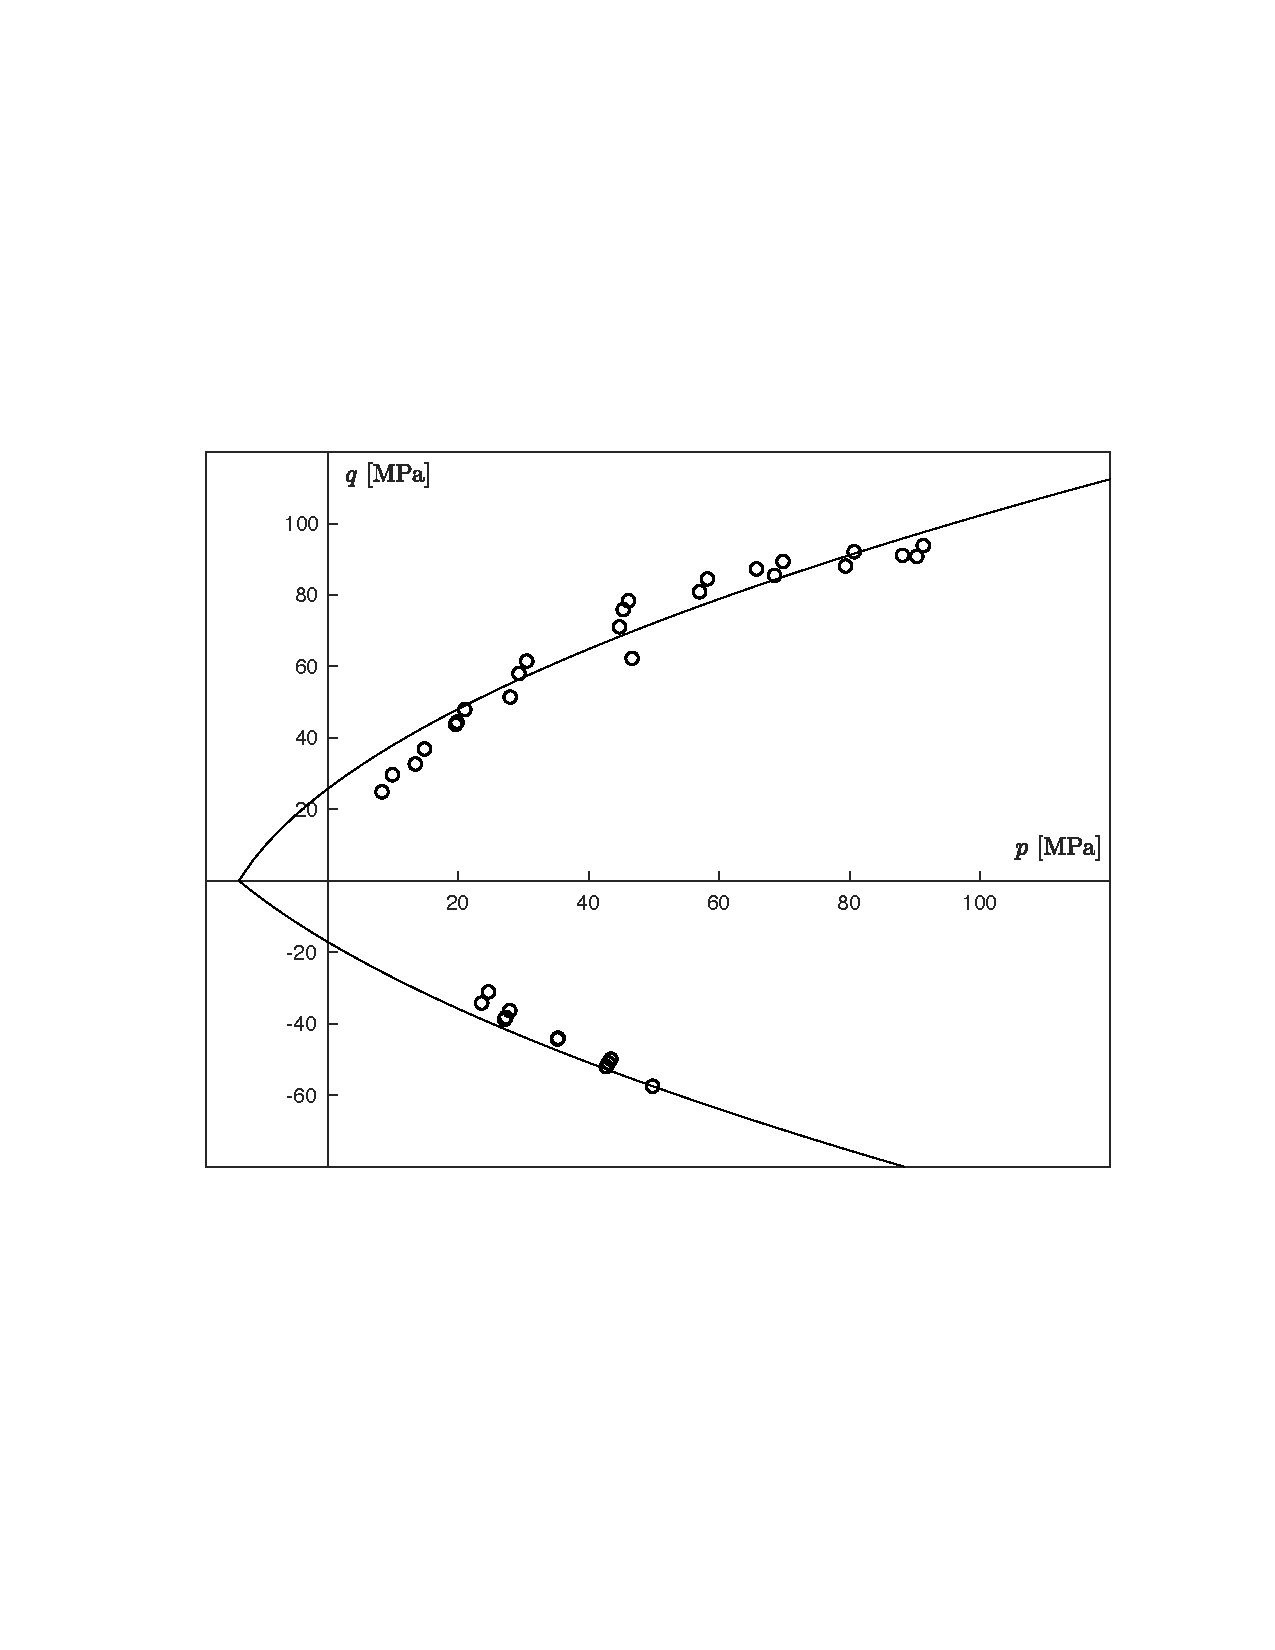
\includegraphics[width=\columnwidth]{ch2/hb_pq}
    \caption{Schematic representation of Hoek-Brown criterion failure surface in $(p-q)$ plane.}
    \label{fig2:hb_pq}
\end{figure} 

\subsubsection{Hoek-Brown in the \texorpdfstring{$\pi$}{pi} plane}\label{ch2:HB_pi}

The Hoek-Brown failure criterion in the $\pi$-plane is presented in Figure \ref{fig2:hb_pi} The failure surfaces can be obtained by inserting Equation \ref{eq2:sig1} and \ref{eq2:sig3} in \ref{eq2:HB-crit}. The obtained expressions and their development are presented in APPENDIX B REF{APPENDIX B}. In Figure \ref{fig2:hb_pi}, the surfaces are exaggerated to show the non-linearity of the criterion.  

\begin{figure}[tb]
    \centering
    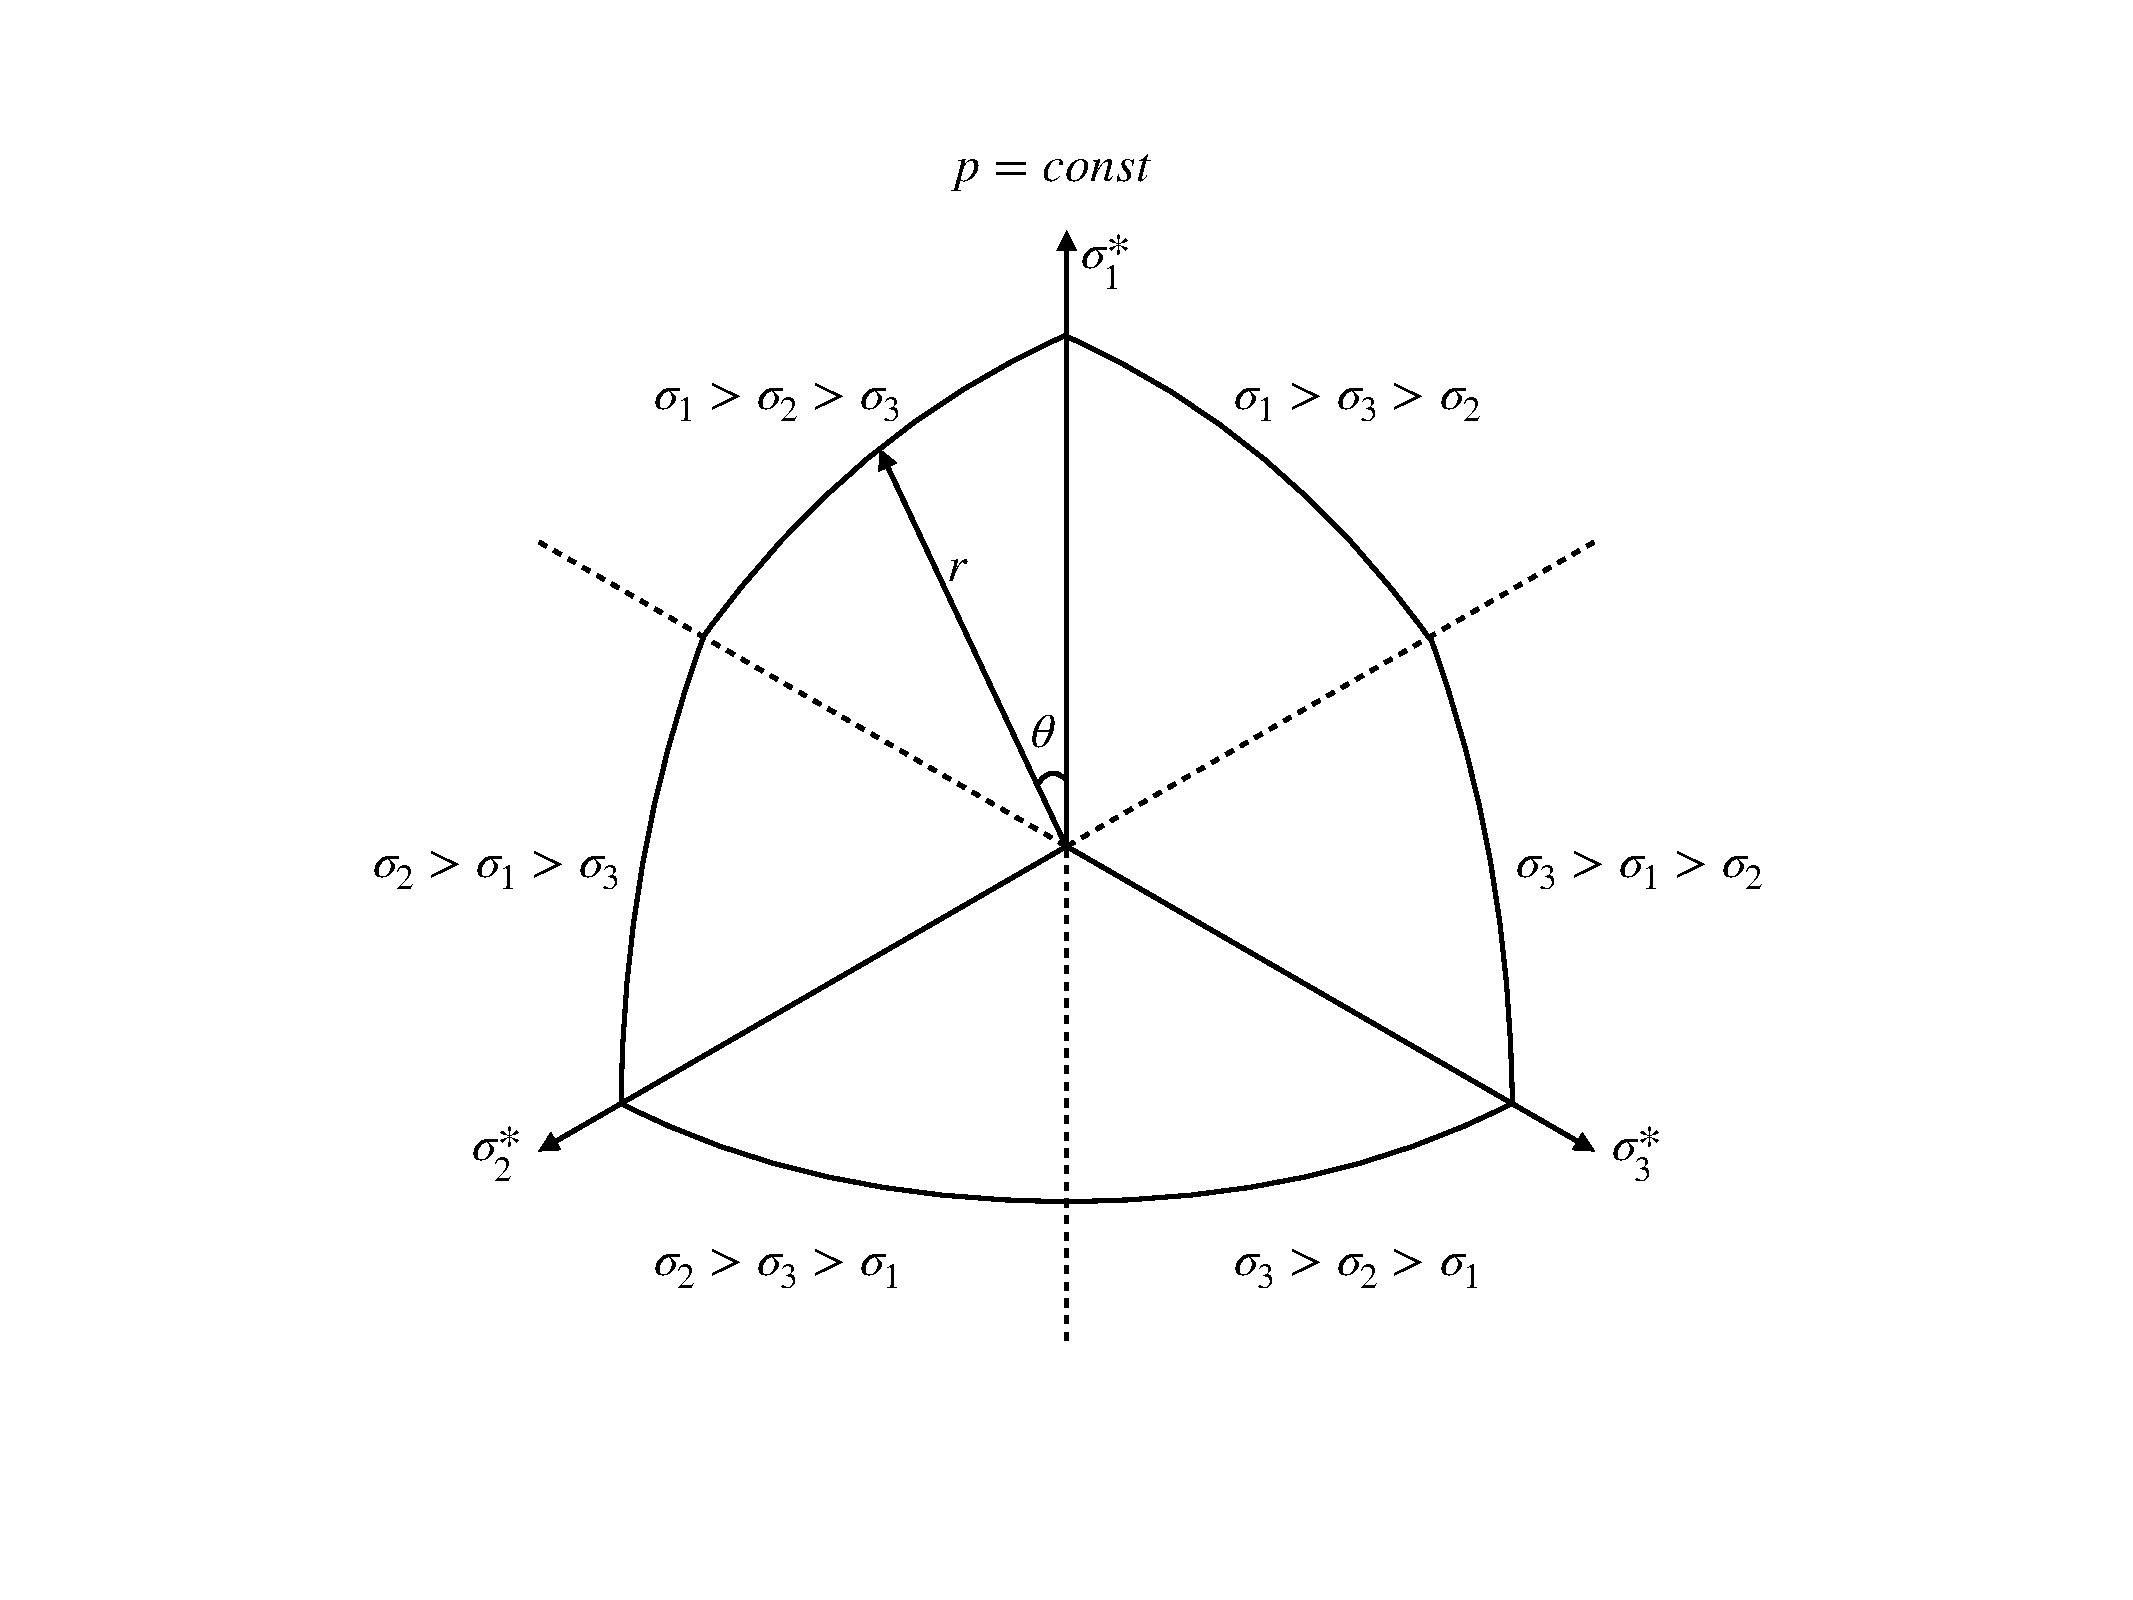
\includegraphics[width=\columnwidth]{ch2/hb_pi}
    \caption{Schematic representation of Hoek-Brown criterion failure surface in $\pi$ plane.}
    \label{fig2:hb_pi}
\end{figure} 

\subsection{Paul-Mohr-Coulomb criterion}\label{ch2:PMC}

The Paul-Mohr-Coulomb criterion (PMC) is a linear model in terms of the three principal stresses. Unlike Mohr-Coulomb and Hoek-Brown, the Paul-Mohr-Coulomb criterion may be used to represent the effect of all principal stresses on rock behavior at failure. Its formulation is based on the one developed by Mohr-Coulomb, for which the intermediate stress effect is added \cite{Paul1968}. The Paul-Mohr-Coulomb failure criterion have the following general expression:

\begin{equation}\label{eq2:PMC}
    A\sigma_I + B\sigma_{II}+C\sigma_{III} = 1
\end{equation}

The ordering of the $A$, $B$ and $C$ with the major, intermediate and minor stresses should be kept as defined in Equation \ref{eq2:PMC}. 

Following Meyer and Labuz (2013) \cite{Meyer2013}, the coefficients A, B and C in terms of the rock properties are expressed as:

\begin{equation}\label{pmc_Acoeff}
    A = \frac{1-\sin \phi_c}{2V_0\sin \phi_c}
\end{equation}
\begin{equation}\label{pmc_Bcoeff}
    B = \frac{\sin \phi_c - \sin \phi_e}{2V_0 \sin \phi_e \sin \phi_c}
\end{equation}
\begin{equation}\label{pmc_Ccoeff}
    C = -\frac{1+\sin \phi_e}{2V_0\sin \phi_e}
\end{equation}

Equation \ref{eq2:PMC} can therefore be written in its complete form as follow:

\begin{equation}\label{eq2:PMC_dev}
    \sigma_{I}\left[\frac{1-\sin \phi_{c}}{2 V_{0} \sin \phi_{c}}\right]+\sigma_{II}\left[\frac{\sin \phi_{c}-\sin \phi_{e}}{2 V_{0} \sin \phi_{e} \sin \phi_{c}}\right]+\sigma_{III}\left[-\frac{1+\sin \phi_{e}}{2 V_{0} \sin \phi_{e}}\right]=1
\end{equation}

PMC refines failure criterion definition by considering different values of the rock properties. It is shown in Equation \ref{eq2:PMC_dev} by the subscripts $c$ and $e$, defining the variables for compression or extension.

\subsubsection{Paul-Mohr-Coulomb in the \texorpdfstring{$(\sigma_3 -\sigma_1)$}{sigma 3 - sigma 1} plane}\label{ch2:PMCsig1sig3}

Paul-Mohr-Coulomb is based on the Mohr-Coulomb criterion, therefore its expression in the $(\sigma_3 -\sigma_1)$ plane is an adjustment of Equation \ref{eq2:PMC_dev} considering different friction angles and cohesion for compression and extension conditions: 

\begin{equation}\label{eq2:PMC_sig1sig3}
    \sigma_I = M_{c,e}\sigma_{III}+C_{c,e}
\end{equation}

Where:

\begin{equation}\label{eq2:PMC_sig1sig3_Mce}
    M_{c,e} = \frac{1+\sin \phi_{c,e}}{1-\sin \phi_{c,e}}
\end{equation}

\begin{equation}\label{eq2:PMC_sig1sig3_Cce}
    C_{c,e} = \frac{2c_{c,e}\cos \phi_{c,e}}{1-\sin \phi_{c,e}}
\end{equation}

Paul-Mohr-Coulomb failure surfaces in $(\sigma_3 -\sigma_1)$ coordinates system are presented in Figure \ref{fig2:pmc_sig1sig3}. As the friction angle and the cohesion for compression and extension are different, Paul-Mohr-Coulomb is not necessarily symmetrical about the hydrostatic axis. The computation of $V_0$ will be discussed in section \ref{ch2:pmcfit}. 

\begin{figure}[tb]
    \centering
    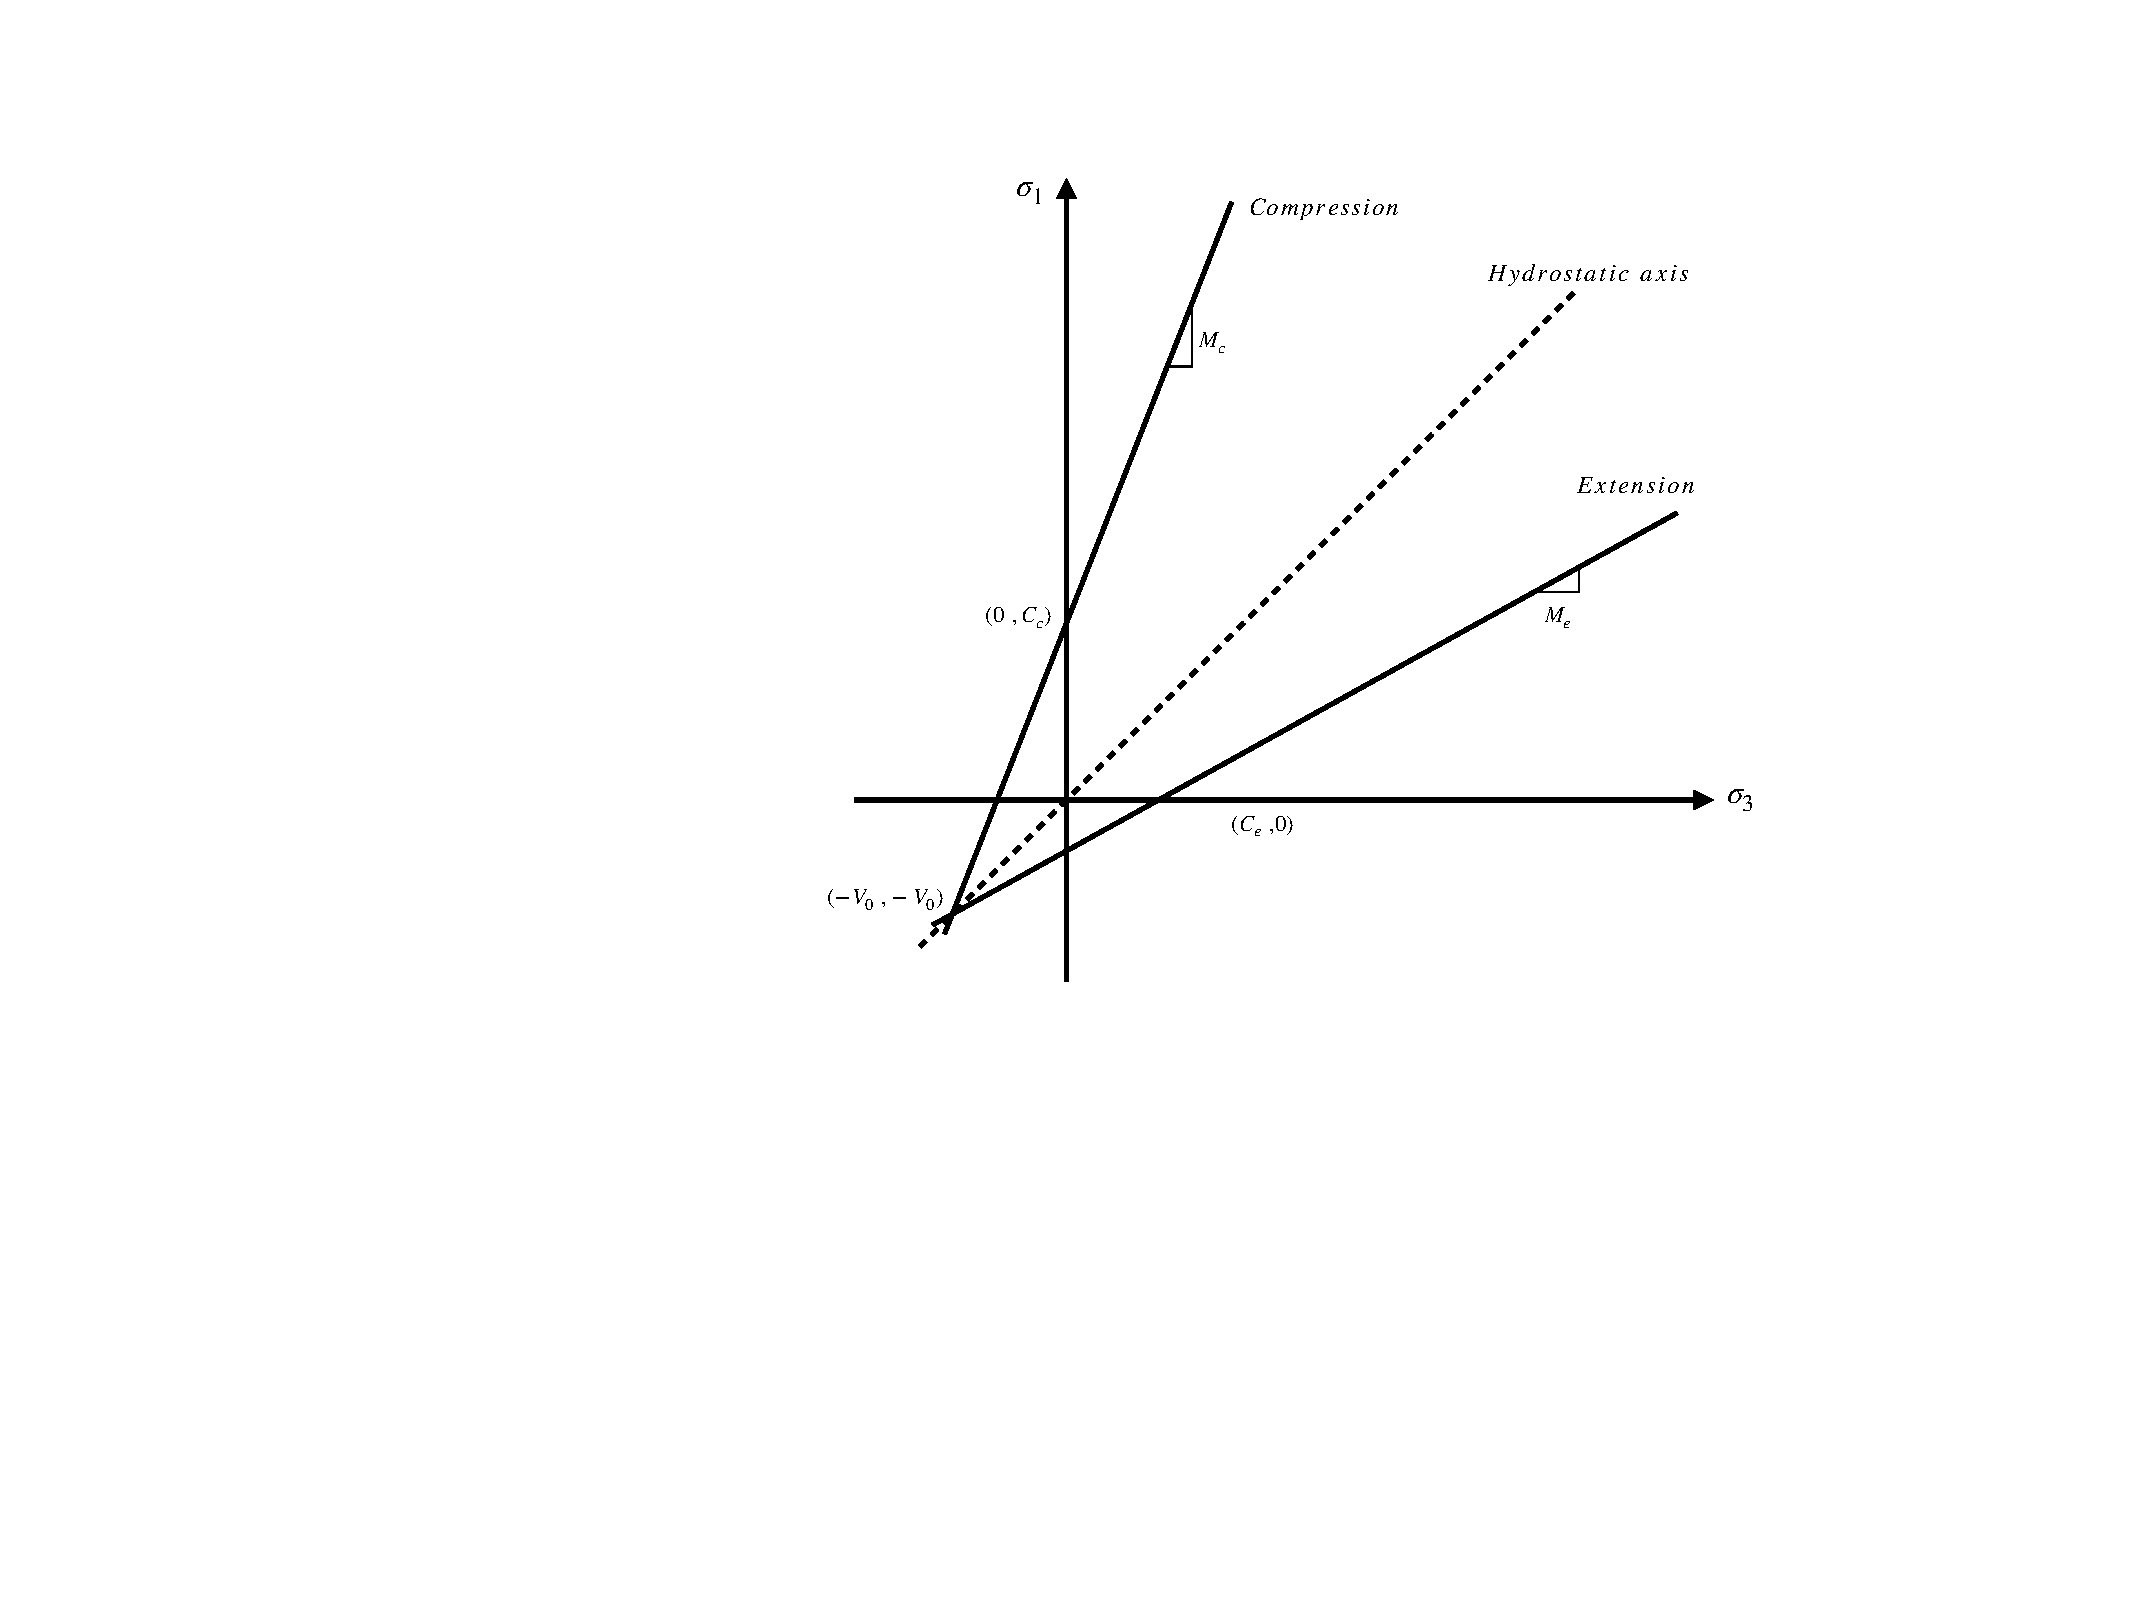
\includegraphics[width=\columnwidth]{ch2/pmc_sig1sig3}
    \caption{Schematic representation of Paul-Mohr-Coulomb criterion failure surface in $(\sigma_3 -\sigma_1)$ plane.}
    \label{fig2:pmc_sig1sig3}
\end{figure} 

\subsubsection{Paul-Mohr-Coulomb in the \texorpdfstring{$(p-q)$}{p-q} plane}

The PMC in the $(p-q)$ coordinate system for axisymmetric loading may be defined as:

\begin{equation}\label{eq2:pmc-q-CTC}
    q_c=\frac{6 \sin \phi_{c}}{3-\sin \phi_{c}} p+\frac{6 c_{c} \cos \phi_{c}}{3-\sin \phi_{c}}
\end{equation}

\begin{equation}\label{eq2:pmc-q-CTE}
    q_e=\frac{6 \sin \phi_{e}}{3+\sin \phi_{e}} p+\frac{6 c_{e} \cos  \phi_{e}}{3+\sin \phi_{e}}
\end{equation}

or in the indicial form as:

\begin{equation}\label{eq2:PMC_pq}
    q = m_{c,e}p+b_{c,e}
\end{equation}

where the coefficients $m_{c,e}$ and $b_{c,e}$ are defined as follow:
\begin{align}\label{eq2:pmc_m_pq}
    m_c=\frac{6 \sin \phi_{c}}{3-\sin \phi_{c}} \quad \textrm{and} \quad m_e=\frac{6 \sin \phi_{e}}{3+\sin \phi_{e}} 
\end{align}
\begin{align}\label{eq2:pmc_b_pq}
    b_c=\frac{6 c_{c} \cos \phi_{c}}{3-\sin \phi_{c}}\quad \textrm{and} \quad b_e=\frac{6 c_{e} \cos \phi_{e}}{3+\sin \phi_{e}}
\end{align}

Figure 2.3 for Mohr-Coulomb can be used to represent Paul-Mohr-Coulomb criterion after $m_{c,e}$ and $b_{c,e}$ recalculated for it.

\subsubsection{Paul-Mohr-Coulomb in the \texorpdfstring{$\pi$}{pi} plane}\label{ch2:PMC_pi}

The representation of the Paul-Mohr-Coulomb failure criterion in the $\pi$-plane is similar to Mohr-Coulomb presented in Figure \ref{fig2:mc_pi}. The failure surfaces can be obtained by inserting Equation \ref{eq2:sig1} and \ref{eq2:sig3} in \ref{eq2:PMC_dev}. The obtained expressions and their development are presented in Appendix %\ref{App:A}. 

\section{Paul-Mohr-Coulomb fitting }\label{ch2:pmcfit}

Failure criterion are conjectural. They try to provide a mathematical formulation of rock behavior based on experiments. However, the results obtained from them are not direct measurements of the friction angle or cohesion. The data from strength testing give the state of stress at failure. The fitting parameters are computed from these stresses.

The use of the Paul-Mohr-Coulomb requires that the model constants ($V_0$, $\phi$) be estimated by fitting the Paul-Mohr-Coulomb criterion to the measured data from conventional triaxial compression, conventional triaxial extension, and true triaxial tests. Labuz et al. \cite{Labuz2018} provide a detailed mathematical derivation of Equations \ref{eq2:sig1} to \ref{eq2:sig3} that leads to the expression of Paul-Mohr-Coulomb failure criterion in terms of the stress invariants $p$, $q$ and $\theta$. 

Failure criterion fitting consist in the computation of the rock properties ($V_0$, $\phi$) from a mathematical formulation of the criterion written in terms of the three principal stresses. Labuz (2018) \cite{Labuz2018} and Folta (2016) \cite{Folta2016} provide detailed mathematical derivation of Equations \ref{eq2:sig1} - \ref{eq2:sig3} that leads to the expression of Paul-Mohr-Coulomb failure criterion in terms of the stress invariants $p$, $q$  and $\theta$. 

The final formulation is given by Equation \ref{eq2:PMCfinalform}:

\begin{equation}\label{eq2:PMCfinalform}
    q\cos(\theta) = \frac{b_c}{V_0}p+k\sin(\theta)q+b_c
\end{equation}

where:
\begin{align}
    k &= \frac{1-2\alpha }{\sqrt{3}}\\
    \alpha &= \frac{b_c}{b_e}
\end{align}

Each data point i from a conventional triaxial or multi-axial experiment is defined by a set of $(p_i,q_i,\theta_i)$ values. Therefore, for any given data set, Equation \ref{eq2:PMCfinalform} describes a system of linear equations. This system has m equations, with m being the number of experiments performed on the rock. Equation \ref{eq2:PMCfinalform} can also be written as a matrix equation of the type $Ax=b$:

\begin{equation}\label{eq2:mat-eq}
    \left[\begin{array}{c}
    {q_{1} \cos \left(\theta_{1}\right)} \\
    {\cdots} \\
    {q_{m} \cos \left(\theta_{m}\right)}
    \end{array}\right]=\left[\begin{array}{ccc}
    {p_{1}} & {q_{1} \sin \theta_{1}} & {1} \\
    {\cdots} & {\cdots} & {\cdots} \\
    {p_{m}} & {q_{m} \sin \theta_{m}} & {1}
    \end{array}\right]\left[\begin{array}{c}
    {b_{c} / V_{0}} \\
    {k} \\
    {b_{c}}
    \end{array}\right]
\end{equation}

where the matrix $A$ is m-by-3, the vector $b$ has m-row, and the vector $x$ has 3-row. 

From the system defined in Equation \ref{eq2:mat-eq}, $b_c$ , $k$, and $V_0$  and can be determined; $k$ and $b_c$  are given by the second and third row of parameter vector $x$, and $V_0$ and $b_e$ are computed as follow: 
\begin{equation}\label{eq2:pmc_vo}
    V_0 = \frac{b_c}{x_1}
\end{equation}
\begin{equation}\label{eq2:pmc_be}
    b_e = \frac{2b_c}{(1-\sqrt{3}k)} 
\end{equation}

The friction angles can be determined by solving Equations for \ref{eq2:pmc-q-CTC} and \ref{eq2:pmc-q-CTE} for $q(p=-V_0)=0$:

\begin{align}\label{eq2:pmc_phi}
    \sin \phi_c &= \frac{3b_c}{6V_0+b_c} \\
    \sin \phi_e &= \frac{3b_e}{6V_0-b_e} 
\end{align}

Similarly, the cohesions are obtained for $q(p=0)=b_{c,e}$:
\begin{align}\label{eq2:pmc_c}
    c_{c} =\frac{b_{c}\left(3-\sin \phi_{c}\right)}{6 \cos \phi_{c}} \\
    c_{e} =\frac{b_{e}\left(3+\sin \phi_{e}\right)}{6 \cos \phi_{e}}
\end{align}